
 % !TEX encoding = UTF-8 Unicode
%% bare_conf.tex
%% V1.4b
%% 2015/08/26
%% by Michael Shell
%% See:
%% http://www.michaelshell.org/
%% for current contact information.
%%
%% This is a skeleton file demonstrating the use of IEEEtran.cls
%% (requires IEEEtran.cls version 1.8b or later) with an IEEE
%% conference paper.
%%
%% Support sites:
%% http://www.michaelshell.org/tex/ieeetran/
%% http://www.ctan.org/pkg/ieeetran
%% and
%% http://www.ieee.org/

%%*************************************************************************
%% Legal Notice:
%% This code is offered as-is without any warranty either expressed or
%% implied; without even the implied warranty of MERCHANTABILITY or
%% FITNESS FOR A PARTICULAR PURPOSE! 
%% User assumes all risk.
%% In no event shall the IEEE or any contributor to this code be liable for
%% any damages or losses, including, but not limited to, incidental,
%% consequential, or any other damages, resulting from the use or misuse
%% of any information contained here.
%%
%% All comments are the opinions of their respective authors and are not
%% necessarily endorsed by the IEEE.
%%
%% This work is distributed under the LaTeX Project Public License (LPPL)
%% ( http://www.latex-project.org/ ) version 1.3, and may be freely used,
%% distributed and modified. A copy of the LPPL, version 1.3, is included
%% in the base LaTeX documentation of all distributions of LaTeX released
%% 2003/12/01 or later.
%% Retain all contribution notices and credits.
%% ** Modified files should be clearly indicated as such, including  **
%% ** renaming them and changing author support contact information. **
%%*************************************************************************


% *** Authors should verify (and, if needed, correct) their LaTeX system  ***
% *** with the testflow diagnostic prior to trusting their LaTeX platform ***
% *** with production work. The IEEE's font choices and paper sizes can   ***
% *** trigger bugs that do not appear when using other class files.       ***                          ***
% The testflow support page is at:
% http://www.michaelshell.org/tex/testflow/



\documentclass[conference]{IEEEtran}
% Some Computer Society conferences also require the compsoc mode option,
% but others use the standard conference format.
%
% If IEEEtran.cls has not been installed into the LaTeX system files,
% manually specify the path to it like:
% \documentclass[conference]{../sty/IEEEtran}





% Some very useful LaTeX packages include:
% (uncomment the ones you want to load)


% *** MISC UTILITY PACKAGES ***
%
%\usepackage{ifpdf}
% Heiko Oberdiek's ifpdf.sty is very useful if you need conditional
% compilation based on whether the output is pdf or dvi.
% usage:
% \ifpdf
%   % pdf code
% \else
%   % dvi code
% \fi
% The latest version of ifpdf.sty can be obtained from:
% http://www.ctan.org/pkg/ifpdf
% Also, note that IEEEtran.cls V1.7 and later provides a builtin
% \ifCLASSINFOpdf conditional that works the same way.
% When switching from latex to pdflatex and vice-versa, the compiler may
% have to be run twice to clear warning/error messages.



% *** CITATION PACKAGES ***
%
\usepackage{cite/cite}
% cite.sty was written by Donald Arseneau
% V1.6 and later of IEEEtran pre-defines the format of the cite.sty package
% \cite{} output to follow that of the IEEE. Loading the cite package will
% result in citation numbers being automatically sorted and properly
% "compressed/ranged". e.g., [1], [9], [2], [7], [5], [6] without using
% cite.sty will become [1], [2], [5]--[7], [9] using cite.sty. cite.sty's
% \cite will automatically add leading space, if needed. Use cite.sty's
% noadjust option (cite.sty V3.8 and later) if you want to turn this off
% such as if a citation ever needs to be enclosed in parenthesis.
% cite.sty is already installed on most LaTeX systems. Be sure and use
% version 5.0 (2009-03-20) and later if using hyperref.sty.
% The latest version can be obtained at:
% \usepackage{amsmath}pkg/cite
\usepackage{amsfonts}
\usepackage{amssymb}



% *** GRAPHICS RELATED PACKAGES ***
%
\ifCLASSINFOpdf
   \usepackage[pdftex]{graphicx}
  % declare the path(s) where your graphic files are
  % \graphicspath{{../pdf/}{../jpeg/}}
  % and their extensions so you won't have to specify these with
  % every instance of \includegraphics
  % \DeclareGraphicsExtensions{.pdf,.jpeg,.png}
\else
  % or other class option (dvipsone, dvipdf, if not using dvips). graphicx
  % will default to the driver specified in the system graphics.cfg if no
  % driver is specified.
  % \usepackage[dvips]{graphicx}
  % declare the path(s) where your graphic files are
  % \graphicspath{{../eps/}}
  % and their extensions so you won't have to specify these with
  % every instance of \includegraphics
  % \DeclareGraphicsExtensions{.eps}
\fi
% graphicx was written by David Carlisle and Sebastian Rahtz. It is
% required if you want graphics, photos, etc. graphicx.sty is already
% installed on most LaTeX systems. The latest version and documentation
% can be obtained at: 
% http://www.ctan.org/pkg/graphicx
% Another good source of documentation is "Using Imported Graphics in
% LaTeX2e" by Keith Reckdahl which can be found at:
% http://www.ctan.org/pkg/epslatex
%
% latex, and pdflatex in dvi mode, support graphics in encapsulated
% postscript (.eps) format. pdflatex in pdf mode supports graphics
% in .pdf, .jpeg, .png and .mps (metapost) formats. Users should ensure
% that all non-photo figures use a vector format (.eps, .pdf, .mps) and
% not a bitmapped formats (.jpeg, .png). The IEEE frowns on bitmapped formats
% which can result in "jaggedy"/blurry rendering of lines and letters as
% well as large increases in file sizes.
%
% You can find documentation about the pdfTeX application at:
% http://www.tug.org/applications/pdftex





% *** MATH PACKAGES ***
%
\usepackage{amsmath}
% A popular package from the American Mathematical Society that provides
% many useful and powerful commands for dealing with mathematics.
%
% Note that the amsmath package sets \interdisplaylinepenalty to 10000
% thus preventing page breaks from occurring within multiline equations. Use:
%\interdisplaylinepenalty=2500
% after loading amsmath to restore such page breaks as IEEEtran.cls normally
% does. amsmath.sty is already installed on most LaTeX systems. The latest
% version and documentation can be obtained at:
% http://www.ctan.org/pkg/amsmath





% *** SPECIALIZED LIST PACKAGES ***
%
%\usepackage{algorithmic}
% algorithmic.sty was written by Peter Williams and Rogerio Brito.
% This package provides an algorithmic environment fo describing algorithms.
% You can use the algorithmic environment in-text or within a figure
% environment to provide for a floating algorithm. Do NOT use the algorithm
% floating environment provided by algorithm.sty (by the same authors) or
% algorithm2e.sty (by Christophe Fiorio) as the IEEE does not use dedicated
% algorithm float types and packages that provide these will not provide
% correct IEEE style captions. The latest version and documentation of
% algorithmic.sty can be obtained at:
% http://www.ctan.org/pkg/algorithms
% Also of interest may be the (relatively newer and more customizable)
% algorithmicx.sty package by Szasz Janos:
% http://www.ctan.org/pkg/algorithmicx




% *** ALIGNMENT PACKAGES ***
%
%\usepackage{array}
% Frank Mittelbach's and David Carlisle's array.sty patches and improves
% the standard LaTeX2e array and tabular environments to provide better
% appearance and additional user controls. As the default LaTeX2e table
% generation code is lacking to the point of almost being broken with
% respect to the quality of the end results, all users are strongly
% advised to use an enhanced (at the very least that provided by array.sty)
% set of table tools. array.sty is already installed on most systems. The
% latest version and documentation can be obtained at:
% http://www.ctan.org/pkg/array


% IEEEtran contains the IEEEeqnarray family of commands that can be used to
% generate multiline equations as well as matrices, tables, etc., of high
% quality.




% *** SUBFIGURE PACKAGES ***
%\ifCLASSOPTIONcompsoc
%  \usepackage[caption=false,font=normalsize,labelfont=sf,textfont=sf]{subfig}
%\else
%  \usepackage[caption=false,font=footnotesize]{subfig}
%\fi
% subfig.sty, written by Steven Douglas Cochran, is the modern replacement
% for subfigure.sty, the latter of which is no longer maintained and is
% incompatible with some LaTeX packages including fixltx2e. However,
% subfig.sty requires and automatically loads Axel Sommerfeldt's caption.sty
% which will override IEEEtran.cls' handling of captions and this will result
% in non-IEEE style figure/table captions. To prevent this problem, be sure
% and invoke subfig.sty's "caption=false" package option (available since
% subfig.sty version 1.3, 2005/06/28) as this is will preserve IEEEtran.cls
% handling of captions.
% Note that the Computer Society format requires a larger sans serif font
% than the serif footnote size font used in traditional IEEE formatting
% and thus the need to invoke different subfig.sty package options depending
% on whether compsoc mode has been enabled.
%
% The latest version and documentation of subfig.sty can be obtained at:
% http://www.ctan.org/pkg/subfig




% *** FLOAT PACKAGES ***
%
%\usepackage{fixltx2e}
% fixltx2e, the successor to the earlier fix2col.sty, was written by
% Frank Mittelbach and David Carlisle. This package corrects a few problems
% in the LaTeX2e kernel, the most notable of which is that in current
% LaTeX2e releases, the ordering of single and double column floats is not
% guaranteed to be preserved. Thus, an unpatched LaTeX2e can allow a
% single column figure to be placed prior to an earlier double column
% figure.
% Be aware that LaTeX2e kernels dated 2015 and later have fixltx2e.sty's
% corrections already built into the system in which case a warning will
% be issued if an attempt is made to load fixltx2e.sty as it is no longer
% needed.
% The latest version and documentation can be found at:
% http://www.ctan.org/pkg/fixltx2e


%\usepackage{stfloats}
% stfloats.sty was written by Sigitas Tolusis. This package gives LaTeX2e
% the ability to do double column floats at the bottom of the page as well
% as the top. (e.g., "\begin{figure*}[!b]" is not normally possible in
% LaTeX2e). It also provides a command:
%\fnbelowfloat
% to enable the placement of footnotes below bottom floats (the standard
% LaTeX2e kernel puts them above bottom floats). This is an invasive package
% which rewrites many portions of the LaTeX2e float routines. It may not work
% with other packages that modify the LaTeX2e float routines. The latest
% version and documentation can be obtained at:
% http://www.ctan.org/pkg/stfloats
% Do not use the stfloats baselinefloat ability as the IEEE does not allow
% \baselineskip to stretch. Authors submitting work to the IEEE should note
% that the IEEE rarely uses double column equations and that authors should try
% to avoid such use. Do not be tempted to use the cuted.sty or midfloat.sty
% packages (also by Sigitas Tolusis) as the IEEE does not format its papers in
% such ways.
% Do not attempt to use stfloats with fixltx2e as they are incompatible.
% Instead, use Morten Hogholm'a dblfloatfix which combines the features
% of both fixltx2e and stfloats:
%
% \usepackage{dblfloatfix}
% The latest version can be found at:
% http://www.ctan.org/pkg/dblfloatfix




% *** PDF, URL AND HYPERLINK PACKAGES ***
%
%\usepackage{url}
% url.sty was written by Donald Arseneau. It provides better support for
% handling and breaking URLs. url.sty is already installed on most LaTeX
% systems. The latest version and documentation can be obtained at:
% http://www.ctan.org/pkg/url
% Basically, \url{my_url_here}.




% *** Do not adjust lengths that control margins, column widths, etc. ***
% *** Do not use packages that alter fonts (such as pslatex).         ***
% There should be no need to do such things with IEEEtran.cls V1.6 and later.
% (Unless specifically asked to do so by the journal or conference you plan
% to submit to, of course. )


\usepackage[english]{babel}
\usepackage[utf8]{inputenc}
\usepackage[T1]{fontenc}
\usepackage{subcaption}
\usepackage{pgfplots}
\usepackage{tikz}
\usetikzlibrary{positioning,decorations.pathreplacing,shapes, automata}
\usepackage{float}

\usepackage{color}
\definecolor{eclipseBlue}{RGB}{42,0.0,255}
\definecolor{eclipseGreen}{RGB}{63,127,95}
\definecolor{eclipsePurple}{RGB}{127,0,85}
\usepackage{listings}
\lstdefinelanguage{htsi}{%
	keywords={for, in, to, if, else, ifEnd, forEnd, True, False},%
	ndkeywords={random, get, set, wait},%
	sensitive=false,%
	morecomment=[l]{#}%
}
\lstset{%
	language={htsi},%
	basicstyle=\small\ttfamily, % Global Code Style
	captionpos=b, % Position of the Caption (t for top, b for bottom)
	extendedchars=true, % Allows 256 instead of 128 ASCII characters
	tabsize=2, % number of spaces indented when discovering a tab 
	columns=fixed, % make all characters equal width
	keepspaces=true, % does not ignore spaces to fit width, convert tabs to spaces
	showstringspaces=false, % lets spaces in strings appear as real spaces
	breaklines=true, % wrap lines if they don't fit
	%frame=trbl, % draw a frame at the top, right, left and bottom of the listing
	%frameround=tttt, % make the frame round at all four corners
	%framesep=4pt, % quarter circle size of the round corners
	numbers=left, % show line numbers at the left
	xleftmargin=1em,%
	numberstyle=\tiny\ttfamily, % style of the line numbers
	commentstyle=\color{eclipseGreen}, % style of comments
	keywordstyle=\color{eclipsePurple}, % style of keywords
	ndkeywordstyle=\color{eclipseBlue},
	%stringstyle=\color{eclipseBlue} % style of strings
}


% correct bad hyphenation here
\hyphenation{op-tical net-works semi-conduc-tor}






\begin{document}
%
% paper title
% Titles are generally capitalized except for words such as a, an, and, as,
% at, but, by, for, in, nor, of, on, or, the, to and up, which are usually
% not capitalized unless they are the first or last word of the title.
% Linebreaks \\ can be used within to get better formatting as desired.
% Do not put math or special symbols in the title.
\title{IT-Security in smart grids:\\Defence strategies for Remote Terminal Units in SCADA networks with limited communication}


% author names and affiliations
% use a multiple column layout for up to three different
% affiliations
\author{
\IEEEauthorblockN{Christof Duhme (421483), Marius Neumann (397664), Thomas Teodorowicz (421489)\\}
\IEEEauthorblockA{Bachelor of Science Informatik\\
Westfälische Wilhelms-Universität Münster}}

% conference papers do not typically use \thanks and this command
% is locked out in conference mode. If really needed, such as for
% the acknowledgment of grants, issue a \IEEEoverridecommandlockouts
% after \documentclass

% for over three affiliations, or if they all won't fit within the width
% of the page, use this alternative format:
% 
%\author{\IEEEauthorblockN{Michael Shell\IEEEauthorrefmark{1},
%Homer Simpson\IEEEauthorrefmark{2},
%James Kirk\IEEEauthorrefmark{3}, 
%Montgomery Scott\IEEEauthorrefmark{3} and
%Eldon Tyrell\IEEEauthorrefmark{4}}
%\IEEEauthorblockA{\IEEEauthorrefmark{1}School of Electrical and Computer Engineering\\
%Georgia Institute of Technology,
%Atlanta, Georgia 30332--0250\\ Email: see http://www.michaelshell.org/contact.html}
%\IEEEauthorblockA{\IEEEauthorrefmark{2}Twentieth Century Fox, Springfield, USA\\
%Email: homer@thesimpsons.com}
%\IEEEauthorblockA{\IEEEauthorrefmark{3}Starfleet Academy, San Francisco, California 96678-2391\\
%Telephone: (800) 555--1212, Fax: (888) 555--1212}
%\IEEEauthorblockA{\IEEEauthorrefmark{4}Tyrell Inc., 123 Replicant Street, Los Angeles, California 90210--4321}}




% use for special paper notices
%\IEEEspecialpapernotice{(Invited Paper)}




% make the title area
\maketitle
\thispagestyle{plain}
\pagestyle{plain}

% As a general rule, do not put math, special symbols or citations
% in the abstract
\begin{abstract}
	
	Power grids are getting rapidly more complex due to increasing quantity of Smart Home Automation, power delivery and even power production units like solar panels. To provide a secure and reliable power grid, intrusion detection systems have to be adapted to these new challenging circumstances. Due to the mentioned complexity the monitoring cannot be done on the top level but has to be moved to a local, decentralized level thus supervising just the local buses is a way to deal with the challenge. This approach will be presented as an implementation in a simulation written for the smart grid co-simulation framework mosaik.

\end{abstract}

% no keywords




% For peer review papers, you can put extra information on the cover
% page as needed:
% \ifCLASSOPTIONpeerreview
% \begin{center} \bfseries EDICS Category: 3-BBND \end{center}
% \fi
%
% For peerreview papers, this IEEEtran command inserts a page break and
% creates the second title. It will be ignored for other modes.
\IEEEpeerreviewmaketitle



\section{Introduction}

	Power grids are controlled through a central based Supervisory Control and Data Acquisition (SCADA) network \cite{chromik1}. It provides the functionality to monitor the system and send commands to remote units to control power flow. Normally, intrusion detection happens on a global level. A possibility is to analyse network traffic behaviour and create a flow whitelist based on the observations \cite{barbosa}. Approaches like this do not consider process-based information and due to rising complexity and non-linear power flow, control and intrusion detection are way to extensive to be done on a global level. \\
	To tackle these problems, decentralising intrusion detection and control mechanisms that consider process-based information, can lead to a more stable, safer and securer network. To achieve this, Remote Terminal Units (RTU) are being located at key nodes where several branches run together. Therefore, the whole grid is controlled and stable if every RTU ensures stability at their own location. The downside of having several RTUs is that new attack possibilities arise, e.g. cyber-attacks used against Ukranian power grids \cite{icscert}. To make RTUs more stable, a local intrusion detections system (IDS) is used at every RTU to enable the RTU to control the power lines, supervised by the RTU, based on the physical values read by the RTU's sensors. To prevent manipulated sensor information from leading to an insecure state, the IDS also validates sensor values with a behaviour specification based approach inspired by rules based on physical information as proposed in \cite{chromik1} and \cite{blithe}. \\
	With the help of the smart grid co-simulation framework mosaik the performance of our IDS is tested by running several types of attack scenarios on several type of smart grids. The process of testing is made easier by our script interpreter, topology loader and improvements to the web visualisation provided by mosaik. The script interpreter enables us to create complex attack scenarios while the topology loader provides a convenient way to switch between different smart grid topologies. \\
	This report contains the following sections. Section 2 introduces smart grid topologies for the simulation. Section 3 details which features we added to the simulation. Section 4 illustrates possible attack types on our smart grid simulation. Section 5 contains test results, their conclusion and ideas for future work.

\section{The scenario}
	
	To simulate a smart grid with mosaik, a topology is needed. Several topologies are introduced that can be used to test the IDS efficiency in various situations.
	
	\subsection{Structure of typologies}
	
		A topology is composed of a grid and any number of RTUs attached to the grid. A grid is composed of a transformer, nodes and branches. The branches connect the transformer to a node from the grid, the nodes among themselves and houses as well as photovoltaic panels to nodes. Houses and photovoltaics (PV) are connected to most but not all nodes. A RTU can be placed at every node. The RTUs monitor the sensors of the nodes they are placed at and also the sensors of the branches connected to the nodes. Furthermore, RTUs are capable of closing and opening the switch of a branch which disables and enables the flow of electricity for the branch respectively.
		
	\subsection{Different topologies}
		
		\begin{figure}[!htp]
			\begin{subfigure}{0.5\textwidth}
				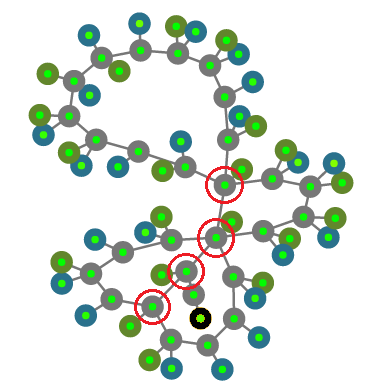
\includegraphics[width=\textwidth]{pics/topo_1_2.png}
			\end{subfigure}
			\underline{Legend:}%
			\begin{itemize}
				\item[] 
\includegraphics[height=15pt]{pics/Node.png} Node
				\item[] \includegraphics[height=15pt]{pics/RefBus.png} RefBus
				\item[] 
\includegraphics[height=15pt]{pics/RTU.png} RTU on a Node
				\item[] 
\includegraphics[height=15pt]{pics/Household.png} Household
				\item[] 
\includegraphics[height=15pt]{pics/PV.png} PV
			\end{itemize}
			\caption{Topology 1 and 1a}
			\label{img:topo_1_2}
		\end{figure}
		
		\begin{figure}[!htp]
			\centering
				\centering
				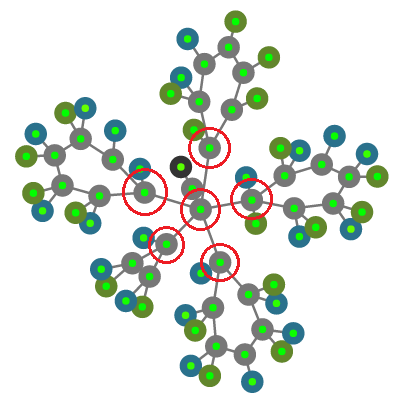
\includegraphics[width=0.5\textwidth]{pics/topo_3.png}
				\caption{Topology 2}
				\label{img:topo_3}
		\end{figure}
	
		\begin{figure}[!htp]
			\centering
				\centering
				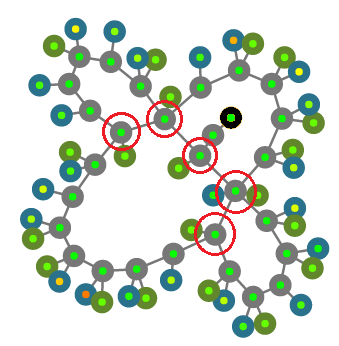
\includegraphics[width=0.5\textwidth]{pics/topo_4_4a.png}
				\caption{Topology 3 and 3a}
				\label{img:topo_4_4a}
		\end{figure}
	
		\begin{figure}[!htp]
			\centering
				\centering
				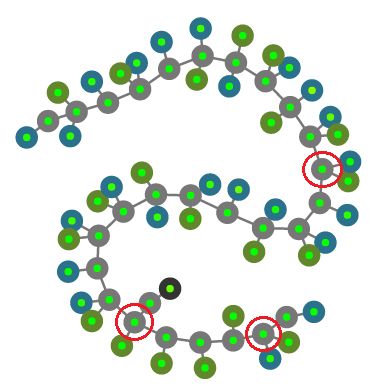
\includegraphics[width=0.5\textwidth]{pics/topo_5.png}
				\caption{Topology 4}
				\label{img:topo_5}
		\end{figure}
		
		\begin{figure}[!htp]
			\centering
				\centering
				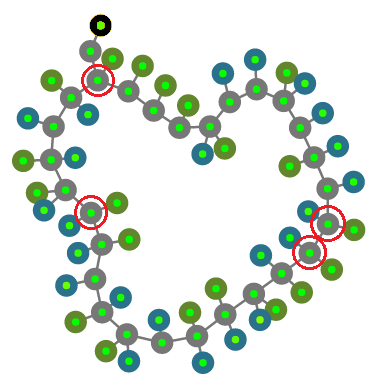
\includegraphics[width=0.5\textwidth]{pics/topo_6.png}
				\caption{Topology 5}
				\label{img:topo_6}
		\end{figure}
	
		We have 7 topologies that all have something unique to them. They are used in combination with attack scenarios to generate data which provides information of the performance of our IDS. It can also be used to fine tune the IDS’s sensitivity. For our default topology we based our grid on a real life grid found in \cite{chromik1} and added RTUs to the 4 most central nodes. This way our IDS can monitor the most crucial points of our grid. The default topology has one parallel	branch which is closed by default and can be opened and closed by the local RTU based on
		certain cut-off values.
		Topology 1a (fig. \ref{img:topo_1_2}) is a clone of our default topology but it includes several RTUs that all supervise a node that posses parallel branches. This topology is used to test which parallel branches are needed and why they are needed or if parallel branches are needed at all. \\
		Topology 2 (fig. \ref{img:topo_3}) has a central node and 5 rings of nodes which are connected to the
		central node by branches. The central node is connected to the transformer. The RTUs are located at the central node and the nodes which are connected with the central node. The purpose of this topology is to test whether we need all 6 RTUs or if we can achieve comparable security by only using one RTU at the central node. \\
		Topology 3 (fig. \ref{img:topo_4_4a}) is composed of a ring of nodes from which one is connected to the	transformer and 4 semicircles. The RTUs are located at the nodes which connect the semicircles with the ring and one at the node which is connected to the transformer. We want to check if our attacks lead to drastically different result when we only change a small part of the topology. Topology 3a is used for similar testing purposes as topology 1a. \\
		Topology 4 (fig. \ref{img:topo_5}) is shaped like a string with one RTU at the node which is connected to the transformer, one RTU at the very end of the string and one RTU at the part of the string where there is no other RTU at the end. The purpose of this topology is to test the communication capabilities of our RTUs and if our RTU would activate the switch when there is no RTU after this one even if this would mean that a part of or grid with multiple households is left without power. \\
		Topology 5 (fig. \ref{img:topo_6}) is shaped like a ring and has a RTU at the node	connecting the ring to the transformer and multiple RTUs on the ring.The purpose of this topology is to further test the communication capabilities of our RTUs. If one RTU decides to
		activate a switch it has to be ensured that no other RTU on the ring also activates a switch because then a part of our grid with multiple households would be left without power.

\section{Implementation in mosaik}
	
	\begin{figure}[!htp]
		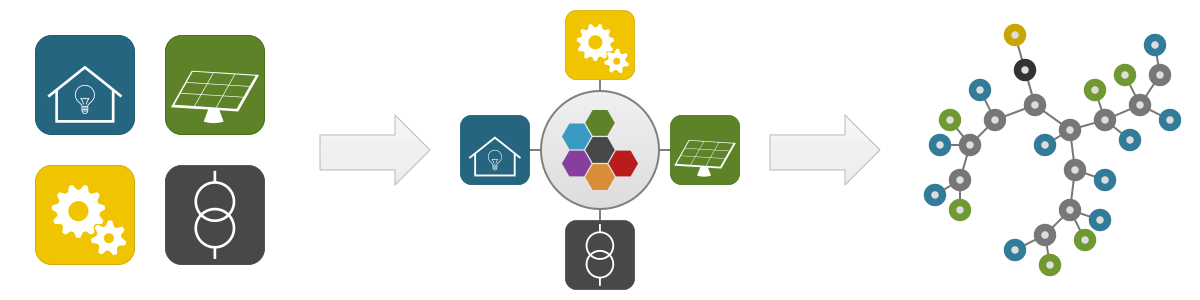
\includegraphics[width=0.5\textwidth]{pics/mosaik-slide.png}
		\caption{Schematic of mosaik's functionality connecting separate simulators to work together. \cite{mosaik}}
		\label{img:mosaik_schematic}
	\end{figure}
	
	Mosaik is a co-simulation framework written in Python and published open source by OFFIS under GNU LGPL \cite{mosaik}. \\
	It provides an API for simulators to implement and then handles the data transfer between them and simulation execution order. \\
	Figure \ref{img:mosaik_schematic} is a simple example and was the base scenario for our work. There are simulators for households (blue), photovoltaics (green), a load flow analysis tool (grey) and a monitoring and analysis tool (yellow). When the simulation is run, the household and PV simulators calculate one step of data. mosaik collects the values and passes them to the flow analysis tool which performs one simulation step. After that mosaik sends the data to the motoring and analysis tool. From there on, these steps are repeated until the simulation is finished. \\
	To manage these interactions, mosaik provides the following components:
	\begin{enumerate}
		\item The \textit{mosaik Sim API} handles the communication between the simulators and mosaik.
		\item The \textit{Scenario API} is for defining the simulation scenario.
		\item The \textit{Simulator Manager} manages the simulator processes and their communication.
		\item mosaik's \textit{simulator} itself is based on the event-discrete simulation library SimPy to execute the scenario simulation.
	\end{enumerate}

	\subsection{Overview}
	
		\begin{figure*}[!htp]
			\centering
			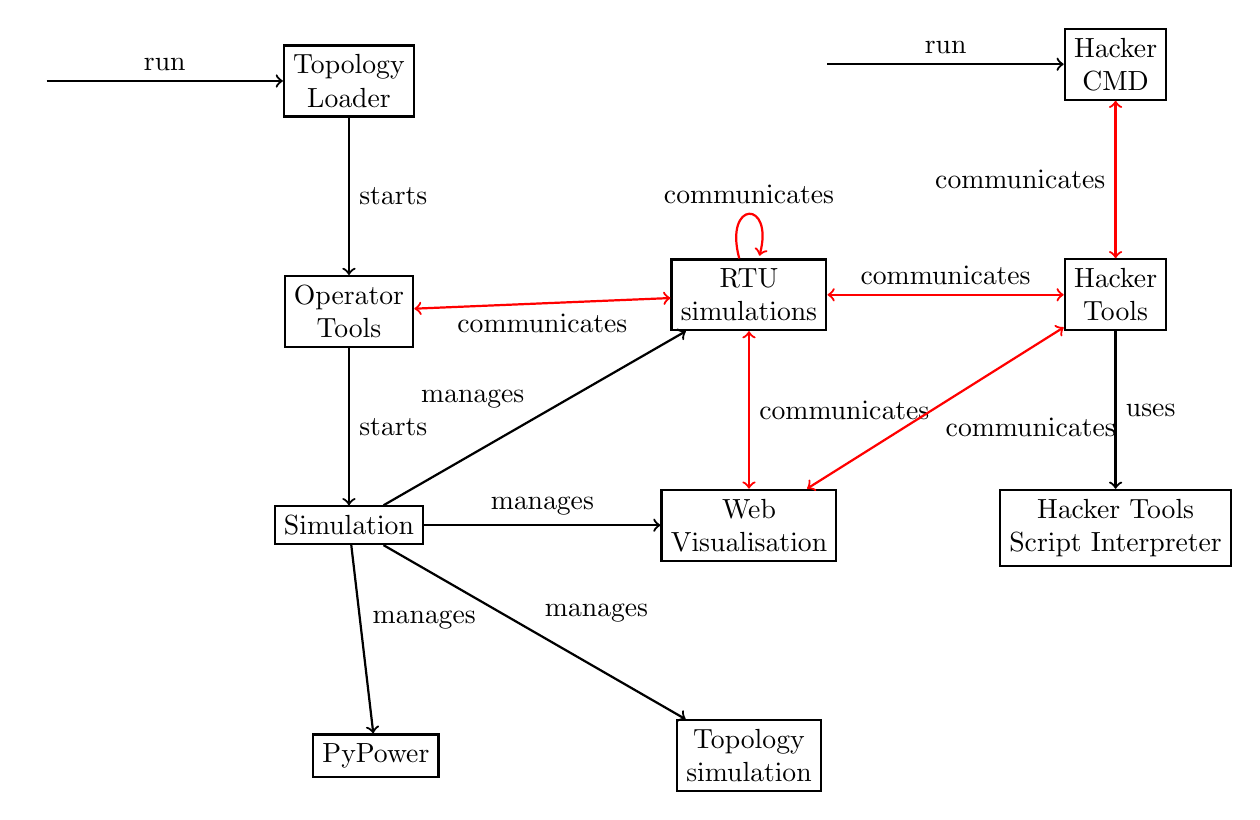
\begin{tikzpicture}[auto, node distance=2cm and 3cm]
				\tikzstyle{class} = [rectangle, draw=black, thick, align=center];
				\tikzstyle{start} = [align=center];
				
				\node[class](topology loader){Topology \\ Loader};
				\node[start, left = of topology loader](start1){};
				\node[class, below = of topology loader](operator){Operator \\ Tools};
				\node[class, below = of operator](simulation){Simulation};
				\node[class, right = of simulation](webvis){Web \\ Visualisation};
				\node[class, below = of webvis](topologysim){Topology \\ simulation};
				\node[class, above = of webvis](RTUsim){RTU \\ simulations};
				\node[class, left = of topologysim](pypower){PyPower};
				\node[class, right = of RTUsim](hackertools){Hacker \\ Tools};
				\node[class, above = of hackertools](hackercmd){Hacker \\ CMD};
				\node[start, left = of hackercmd](start2){};
				\node[class, below = of hackertools](htsi){Hacker Tools \\ Script Interpreter};
				
				\path[draw=black, thick, ->] (topology loader) edge node{starts} (operator)
				(operator) edge node{starts} (simulation)
				(simulation) edge node{manages} (RTUsim)
				(simulation) edge node{manages} (webvis)
				(simulation) edge node{manages} (topologysim)
				(simulation) edge node{manages} (pypower)
				(hackertools) edge node{uses} (htsi)
				(start1) edge node{run} (topology loader)
				(start2) edge node{run} (hackercmd);
				
				\path[draw=red, thick, <->] (RTUsim) edge node{communicates} (hackertools)
				(RTUsim) edge node{communicates} (operator)
				(RTUsim) edge node{communicates} (webvis)
				(RTUsim) edge [loop above] node{communicates} (RTUsim)
				(hackertools) edge node{communicates} (hackercmd)
				(hackertools) edge node{communicates} (webvis);
			\end{tikzpicture}
			\caption{The diagram shows an overview over the structure of the simulation and the communication and management of the subsimulations and external packages.}
			\label{diag:overview}
		\end{figure*}
	
		The diagram \ref{diag:overview} shows the overall structure of the simulation and how the individual packages and classes work together. \\
		The following features were implemented by us. A topology loader for easier switching between scenarios, simulations for every RTU that can communicate with each other, an IDS that is used by the RTUs, improvements to the web visualisation for easier scenario testing, tools for trusted operators and a hacker client to either manually carry out attacks or to execute attack scripts. These features are used for either the simulation itself or for tests concerning the IDS safety.\\
		When running the simulation, the Topology Loader is started first. It provides a GUI for choosing a topology and configuring some simulation parameter. After that the Operator Tools start a GUI for the user to monitor RTU messages and resetting them. It also starts the simulation itself. The simulation persists of the RTU and topology simulation, PyPower for the physics calculations and the Web Visualisation. \\
		When the Hacker CMD is run, it starts the Hacker Tools which handles the communication with the RTU simulation and the Web Visualisation. For executing attack scripts, the Hacker Tools use the Hacker Tools Script Interpreter for translation of the commands to function calls.
	
	\subsection{Topology loader}
		
		Working with different topologies to test the defence algorithms can be exhausting and annoying because every time either multiple files or several paths in the code had to be changed. As a quality of life improvement the topology loader was introduced. It needs every topology to have a configuration file that declares all needed files and directories. There is also the possibility to choose the default settings so large standard files like the PV production table do not need to be copied several times. This prevents the overall size of the data from blowing up. \\
		The loader also provides a graphic user interface (GUI) to select a topology. It also shows an image of the topology layout to make the selection process easier.
	
	\subsection{RTU simulation}
		
		There are multiple RTUs in the grid so the simulation has to simulate all of them. Therefore, more than one RTU simulation has to be started. mosaik gives a parameter option for this but due to a hard coded $1$ in the source code, this possibility cannot be used. So there can only be one RTU simulation. To still simulate a various number of RTUs in a power grid, the RTU simulation class is used as a wrapper for the real simulation. It creates a new thread for each RTU and lets them run independently. It also forwards the simulation data to them in every simulation step.
		
	\subsection{Intrusion Detection System}
		
		The IDS is based on the requirements and physical laws suggested in \cite{chromik1}. \\
		RTUs use R2 and R4 as defined in \cite{chromik1} to regulate the smart grid state of the branches monitored by itself. R2 is the rule that power lines have a max current that is not to be exceeded and R4 requires that if the current of a branch exceeds a cut-off current a second branch, if existing, is opened. As we do not know if commands are trusted, commands are prevented from being executed if R2 or R4 are not violated. To validate sensor values we use a behaviour specification based IDS as suggested in \cite{chromik2} as it can deal with unknown attacks and yields a low false negative rate. Our basis are internal trust values (ITV) assigned to each sensor. If an ITV surpasses a cut-off value we mark a sensor as untrusted. The RTU broadcasts to other RTUs if a sensor was marked as untrustworthy. Untrusted sensors will be ignored until an operator resets the trust. Inspired by \cite{blithe} we check for voltage angle and voltage magnitude at nodes, current at lines that the margin of values of two successive steps do not exceed a cut-off value. If the cut-off value is exceeded we increase the ITV to it's cut-off value. As advised in \cite{blithe} the cut-off principle is implemented for the voltage angle margin between adjacent RTUs. As suggested in \cite{blithe} warnings and great-warnings are given if a margin reaches a percentage of the cut-off value. Warnings and great-warnings increase the ITV in amounts smaller than the cut-off value. This prevents single outliers to lead to marking sensors as untrustworthy. Warnings allow several, smaller outliers while great-warnings allow for less, bigger outliers. To increase adaptability to different smart grids cut-off values and the standard increases to the ITV are easily modifiable. In combination with the ITV, RTUs check R1 and P1 as defined in \cite{chromik1} to validate sensor data. If R1 or P1 are breached by a sensor it's ITV are increased. R1 demands that the voltage on all lines stays within the boundaries 230V +-10\% in low voltage areas. In our simulation we used 10000V as we simulate a middle voltage area. \\
		A notable point about P1, known as Kirchhoff's Law, is the way how it is calculated.
		For example, if there is a node with four branches $a$, $b$, $c$ and $d$ connected, the formula for Kirchhoff's Law with $I_i$ as the current on branch $i$ looks like this presuming the combination of branches is the valid one:
		\begin{equation}
			(I_a + I_b) - (I_c + I_d) = 0
			\label{eq:klaw}
		\end{equation}
		To change the values without violating Kirchhoff's Law, this constraint with $\delta$ indicating the value change between two discrete points in time has to be met:
		\begin{equation}
			\delta I_a + \delta I_b = \delta I_c + \delta I_d
		\end{equation}
		It assures that the equation \ref{eq:klaw} stays true. Because we do not know the flow direction of the current, the only way to get an equation like \ref{eq:klaw} is by trial and error. This is done by checking which combination of signs yields the sum closest to zero. If there is no value close to zero, P1 is violated. The reason why we check for the sum to be only close to zero and not equal is that we are missing the data of PVs and households to consider in the calculations. \\
		For every branch exists a sensor which means that several sensors are on the same node and belong to the same RTU. RTUs check if every sensor at a node reads the same value. If they do not share the same value we mark every sensor at the node as untrusted. As suggested by Prof. Remke, we also added the possibility to use majority rule instead. Our system yields a higher false positive rate if a minority of sensors is attacked while the majority rule yields a higher false negative rate if the majority of sensors is attacked. \\
		Considering this and the adaptability for different smart grids, our IDS design allows to easily switch off or swap out features.		
	
	\subsection{WebVis}
		
		The web visualisation was previously handled by an executable but was changed to python script for easier adjustments. \\
		When being started the web server provides the HTML main page for the browser and through that the JS script which handles the network visualisation by the 3d.js framework and updating the data given by the simulation over the web server. \\
		The server also manages the visual representation of hacker attacks and RTU interventions. The data for this feature is sent to the JS script along with the simulation data. These visualisations are helpful to understand the extent of an attack and the defence behaviour of the RTUs.

	\subsection{Hacker Tools}
		
		To simulate attacks on the grid, it is assumed that the hacker has already gained access to the network e.g. by bypassing a firewall or infecting a PC with a defected USB key.
		
		\subsubsection{Hacker Tools CMD}
			
			For I/O a simple command line shell is used with a limited set of commands. The hacker can connect to RTUs, read the current state of specific branches and send malicious data to override real sensor data with the provided commands. Furthermore, switches on the branches can be turned on and off resulting in a real change of the grid in contrast to the sensor data manipulation which just misleads the IDS. \\
			The data transfer works over the TCP protocol. The server on the RTUs provide a TCP server with a distinct IP address onto which the Hacker Tools can connect with a TCP client. \\
			The link to the web visualisation works in the same way over a TCP based server-client connection. \\
			These clients each run in a separate thread to guarantee responsiveness and let the main thread run even when waiting for a response.
			
		\subsubsection{Script Interpreter}
		
			To automate complex attacks, a script interpreter was added for easy and even intelligent attacks. The used script language is self-developed and simple to learn for ease of use.\\
			The interpreter can handle all normal Hacker Tools commands and following constructs and functions:
			\begin{itemize}
				\item set and get for variables
				\item if - then - else
				\item for-loop
					\begin{itemize}
						\item over a range of values
						\item over an array
					\end{itemize}
				\item random-function
					\begin{itemize}
						\item number in range
						\item element from array
					\end{itemize}
				\item array length function
				\item wait function (waits a given amount of seconds)
			\end{itemize}
			It can calculate $+$, $-$, $*$, $/$ and $mod$. The comparators $==$, $>$, $<$, $>=$, $<=$, $!=$ can be used with logic functions $and$ and $or$. \\
			To make reviewing the script easier, it allows to insert line comments with $\#$ as a token.
			
			\begin{figure}[!htp]
				\lstinputlisting{scripts/randomrtu.txt}
				\caption{Example attack script for a random style attack.}
				\label{script:random}
			\end{figure}
			Figure \ref{script:random} is an example for an attack script. It executes a random attack on the grid by connecting to a random RTU, iterating through all its branches and changing the sensor values by a randomly chosen percentage. Additionally, the decision whether the change is positive or negative is also randomized.
			
			\begin{figure}[!htp]
				\lstinputlisting{scripts/increaseall.txt}
				\caption{Example attack script for increasing all sensor values continuously.}
				\label{script:increaseall}
			\end{figure}
			The attack script in figure \ref{script:increaseall} iterates through all RTU servers and their branches 1000 times. It then increases the branches sensor value by one per cent.
			
	\subsection{Operator Tools}
		
		The Operator Tools provide a simple GUI for hard resetting the local IDSs by making every sensor trusted. It also gives an overview over detected attacks whether true or false positives. It shows all notifications when an RTU's defence mechanism gets triggered.

\section{Attack scenarios}

	When attacking the grid, the hacker has several options on how to structure their attack. They range from simple straight forward to complex and IDS targeted ones.
	
	\subsection{Deterministic attacks}
	
		Deterministic attacks are the easiest to implement because we can list all RTUs in the simulation with the help of Hacker Tools, connect to them and get the data read by their sensors. This enables us to start specific attacks on a single or more RTUs, which can alter specific physical values read by specific sensors of these RTUs or open/close specific switches. For example one could connect to a RTU via the TCP connection and increase a physical value, read by a sensor of this RTU, by a specific amount.
		
	\subsection{Random attacks}
	
		Random attacks try to abuse that they have no pattern, which is not a problem for our IDS as it is not based on pattern recognition. For example we could connect to a random RTU, add a random number to a physical value read by a random amount of sensors of this RTU and then repeat the whole process.
		
	\subsection{Defence mechanism specialized attacks}
	
		Attacks that are engineered to bypass certain defence mechanisms. These attacks require the attacker to know which defensive mechanism are implemented to secure the system.
	
		\begin{enumerate}
			\item For example if the attacker wants to bypass the Kirchhoff’s law he could use an attack on the lines of connecting to a certain RTU, increase the voltage angle value of half of the sensors and	decrease the other sensor’s voltage angle values by the same amount. In theory these attacks easily circumvent our IDS but they not only require knowledge about how our IDS works but also knowledge of the specific cut-off values used.
			
			\item Another approach is to increase the sensor data just by a fraction of its value. This prevents the IDS from triggering its control mechanism because the change of the sensor's value seems to be a normal gradient. When the value reaches the maximal current, the branch will be turned off with no real world reason to do so. This way, drastic changes can be made to the grid without the IDS interfering.
		\end{enumerate}
	
		All IDS defence mechanisms have to be considered to make a successful attack, as different mechanisms cover each other. E.g. you cannot trick the gradient check without also tricking Kirchhoff's Law.
		
	\subsection{Attack to kill the IDS}
		
		Instead of trying to trick the IDS we can also prevent the IDS from checking for an attack. To make this possible, a first attack is run, that will definitely be detected so the IDS will mark those nodes as unsafe. Due to this, these nodes will be ignored by the IDS. This impairs the IDS's control functions, meaning that power lines are not turned off if they exceed their maximally allowed current nor will parallel branches be utilized to reduce their main branches load. At this point we cannot guarantee the grids stability.

\section{Discussion}

	To discuss the work, there is an evaluation at first. After that, we draw a conclusion to our findings and take a look at future work to be done afterwards.
	
	\subsection{Evaluation}
	
		To evaluate our IDS we compare the effect of specific and randomized attacks. They are tested with topology 1 (fig. \ref{img:topo_1_2}).
		
		\subsubsection{Specific attack}
		
			\begin{figure}[!htp]
				\centering
				\begin{tikzpicture}
					\begin{axis}[width=0.5\textwidth, xlabel={time [t]}, ylabel={I\_real [A]}, legend style={font=\fontsize{6}{6}\selectfont}]
						\addplot table [y=sensor_2, mark=none] {stats/topo1/normal/I_real_all.txt};
						\addplot table [y=sensor_2, mark=none] {stats/topo1/spec/I_real_all.txt};
						\addplot table [y=sensor_4, mark=none] {stats/topo1/normal/I_real_all.txt};
						\addplot table [y=sensor_4, mark=none] {stats/topo1/spec/I_real_all.txt};
						\legend{{sensor 2, normal}, {sensor 2, attack}, {sensor 4, normal}, {sensor 4, attack}}
					\end{axis}
				\end{tikzpicture}
				\caption{The plot shows I\_real value against simulation time. For sensor 2 and sensor 4 the values are displayed for both, a normal simulation execution and a simulation where a specific attack was made.}
				\label{plot:atk_spec}
			\end{figure}
		
			\begin{figure*}[!htp]
				\centering
				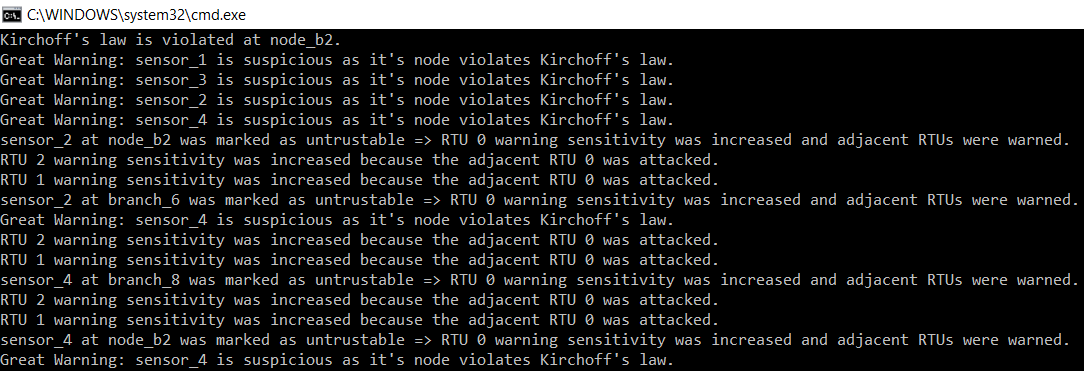
\includegraphics[width=\textwidth]{stats/topo1/spec/topology1_attacked.png}
				\caption{CMD output for the specific attack}
				\label{img:cmd_spec}
			\end{figure*}
		
			This attack increases the current of $branch_2$ and $branch_4$ by 1 per cent each simulation step which is similar to the attack in figure \ref{script:increaseall}. In figure \ref{plot:atk_spec} this continuous increase can be seen as a steady rising of the black and red graph. The attack started at simulation time $47700$ and the IDS triggered great warnings for Kirchhoff's Law immediately. After 3 simulation steps, the attacked sensors warning values reach the unsafe status, meaning the IDS detected the attack. As the attack was detected by the violation of Kirchhoff's Law all sensors on the attacked node were marked as unsafe. Therefore we have two false positives in this scenario. \\
			Figure \ref{img:cmd_spec} shows an example IDS output when an attack is detected.

		\subsubsection{Random attack}
		
			\begin{figure}[!htp]
				\centering
				\begin{tikzpicture}
					\begin{axis}[width=0.5\textwidth, xlabel={time [t]}, ylabel={I\_real [A]}]
						\addplot table [y=sensor_1, mark=none] {stats/topo1/rand/I_real_all.txt};
						\addplot table [y=sensor_2, mark=none] {stats/topo1/rand/I_real_all.txt};
						\addplot table [y=sensor_3, mark=none] {stats/topo1/rand/I_real_all.txt};
						\addplot table [y=sensor_4, mark=none] {stats/topo1/rand/I_real_all.txt};
						\addplot table [y=sensor_5, mark=none] {stats/topo1/rand/I_real_all.txt};
						\addplot table [y=sensor_6, mark=none] {stats/topo1/rand/I_real_all.txt};
						\addplot table [y=sensor_7, mark=none] {stats/topo1/rand/I_real_all.txt};
						\addplot table [y=sensor_8, mark=none] {stats/topo1/rand/I_real_all.txt};
						\addplot table [y=sensor_9, mark=none] {stats/topo1/rand/I_real_all.txt};
						\addplot table [y=sensor_10, mark=none] {stats/topo1/rand/I_real_all.txt};
						\addplot table [y=sensor_11, mark=none] {stats/topo1/rand/I_real_all.txt};
						\addplot table [y=sensor_12, mark=none] {stats/topo1/rand/I_real_all.txt};
						\addplot table [y=sensor_13, mark=none] {stats/topo1/rand/I_real_all.txt};
						\addplot table [y=sensor_14, mark=none] {stats/topo1/rand/I_real_all.txt};
						\addplot table [y=sensor_15, mark=none] {stats/topo1/rand/I_real_all.txt};
						\addplot table [y=sensor_16, mark=none] {stats/topo1/rand/I_real_all.txt};
						\addplot table [y=sensor_17, mark=none] {stats/topo1/rand/I_real_all.txt};
						%\legend{1, 2, 3, 4, 5, 6, 7, 8, 9, 10, 11, 12, 13, 14, 15, 16, 17}
					\end{axis}
				\end{tikzpicture}
				\caption{The plot shows I\_real value against simulation time. A graph is shown for every sensors value during a simulation where a random attack was executed.}
				\label{plot:atk_rand}
			\end{figure}
			
			This attack is the one presented in (fig. \ref{script:random}. It randomly picks a RTU, then randomly picks a sensor and then changes the value read by the sensor by a random percentage either positive or negative in the range between 25 and 75. Due to this the graphs in the plot (fig. \ref{plot:atk_rand}) look like step functions. It is notable that one branch does not appear to have been chosen for an attack during this run of the simulation. Before even drastic jumps can trigger gradient checks, Kirchhoff's Law detects the intrusion.
			
		\subsection{Conclusion}

			Due to the severe consequences that attacks on smart grids can have, the security is the top priority with current approaches not being comprehensive enough to cover every potential attack possibility. This work tests the performance of a local system that acts based on locally attainable physical information. \\
			We discovered that it is very complicated to bypass Kirchhoff's Law.
			Like our IDS an attacker cannot separate in- and output branches of a node. Due to this, the attacker has to do the same calculations as the IDS to determinate current flow directions. Only then he can successfully evade Kirchhoff's Law. This makes Kirchoff's Law a strong point of our IDS. \\
			We also noted that the cut-off values used in our attack scenarios are too high to trigger an unsafe marking as Kirchhoff's Law is too accurate.\\
			As a conclusion we consider neither deterministic nor random attacks to be sufficient enough to harm the grid without the IDS noticing.\\
			Especially Kirchhoff's Law prevents these attack types by definition.\\
			As Kirchhoff's Law is more sensitive than expected and by declaring all sensors at a node unsafe when a violation is detected, we get many false positives. Therefore, we conclude that using the majority rule feature instead we can reduce the amount of false positives while not increasing false negatives except for attacks targeted against this defence mechanism. \\
			Test results show that using a local system that acts on process-based information is able to consistently detect several types of attacks while having a low amount of false positives. However, attacks that abuse knowledge of the behaviour specifications are expected to be successful. 
	
	\subsection{Future work}
		
		Although a lot of work was done in this project, there are still some things to consider for improvement and more functionality. \\
		At the moment, all nodes in a grid are treated the same way. But the first node after the reference bus is exposed to a much greater current than all the other ones. A special treatment for nodes like that would be great addition, so the sensitivity for normal nodes can be increased. On a similar note the current generally decreases the further away a node is from the reference bus which could be used to fine tune more distant RTUs with smaller cut-off values. \\
		When handling commandos we use a very restricted system. The first problem is that suspicious commands are not prevented from being executed but we only execute a reverse command in the next step. Ideally we would prevent suspicious commands from being executed in the first place. Another problem is that commands are not checked at all if an untrusted sensor has to be checked to validate the command. Handling this problem in a more complex way, e.g. something like a pattern recognition to filter out greater chunks of commands that are not harmful alone but all together, would increase the system's safety. \\
		Currently a RTU cannot get the current readings of PVs and households. This results in rather inaccurate calculations such as the check for Kirchhoff's Law, for example. Getting these values would drastically improve the simulation because there would be no need to round and estimate results. \\
		At the moment our IDS is rather easily tricked by gradually increasing and decreasing current values read by branch sensors on a single node in a way that Kirchhoff's Law is not violated at the node. This leads to closing of power lines as soon as they exceed the maximally allowed current. Therefore, it would be interesting to see if pattern based detection methods would be a good extension for our current IDS. \\
		Additionally, when a real error occurs on a node that was marked as unsafe, this is neither detected nor handled. For sensors on a node this may be able to be fixed with a system, that automatically restores trust for a sensor when it's read data values are matching the other node's sensor's readings for a certain amount of time. \\
		In \cite{chromik1} other requirements and physical laws were defined which we either could not implement, did not need to implement or did not have the time to implement. P2 and P4 are restricted by the simulation. Lines that are turned of to not have zero current within the simulation so P2 cannot be checked. To realize P4 we need to know the voltage from power lines. As we could not attain this value we did not implement P4. R3 cannot be checked because we are missing the source power production values. This is due to the fact that the simulation does not contain these but just equals power loads out at the reference bus. P5 and P6 concerned transformers which are not the focus of our group. P3 could be implemented if we get the specific branch data, e.g. it's length, and check if the two power values given at a branch are the same after considering the resistances. \\
		As for the Hacker Tools Script Interpreter, a great improvement would be an error detection system that handles syntactical mistakes so the whole Hacker Tools shell does not crash every time.

\bibliographystyle{IEEEtran}
\bibliography{paper_bib}

% that's all folks
\end{document}
